% !TEX root = ../Projektdokumentation.tex
\section{Analysephase} 
\label{sec:Analysephase}


\subsection{Ist-Analyse} 
\label{sec:IstAnalyse}
Derzeit haben Mieter eines ePages-Onlineshops die Möglichkeit im Backoffice ihres Onlineshop, in dem alle wichtigen Shopeinstellungen zu treffen sind, zwei Analysewidgets auszuwählen. Das erste zeigt eine Top-3-Liste der meistverkauften Artikel der letzten 30 Tage an und das zweite den Nettoumsatz sowie die Anzahl der Bestellungen für heute, gestern, diese Woche, letzte Woche, diesen und letzten Monat an.
\begin{figure}[htb]
\begin{center}
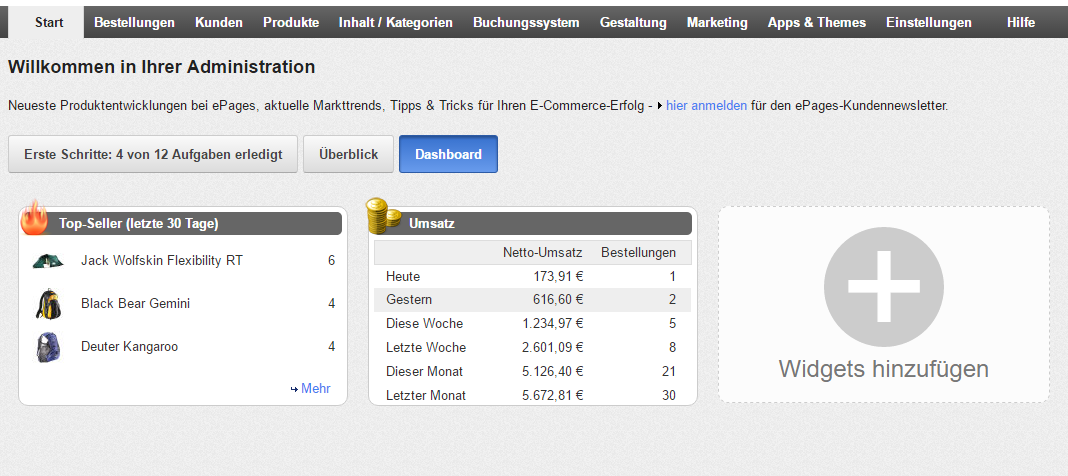
\includegraphics[width=0.9\textwidth]{dashboard.png}
\end{center}
\end{figure}
Des Weiteren wurde bereits auf einem zweitägigen firmeninternen Hackathon im Frühjahr 2016 der Versuch der Programmierung einer Statistik-App unternommen, wobei dabei nur mit "Mock-Daten" hantiert wurde und keine echte Shopanbindung realisiert wurde. Die Ergebnisse zu dieser App sind auf einer internen Wikiseite veröffentlicht und liefern einen ersten Eindruck wie so eine App aussehen könnte und welche Funktionalitäten und Use-Cases ePages vorrangig für solch eine Statistik-App vorsieht.

\subsection{Wirtschaftlichkeitsanalyse}
\label{sec:Wirtschaftlichkeitsanalyse}

\subsubsection{\gqq{Make or Buy}-Entscheidung}
\label{sec:MakeOrBuyEntscheidung}

Für jeden Endkunden einen ePages-Onlineshops besteht bereits die Möglichkeit über interne kostenlose Widgets den täglichen, wöchentlichen oder monatlichen Umsatz oder die für diese Zeiträume getätigten Bestellungen angezeigt zu bekommen. Zusätzlich können letzte Kundenregistrierungen und letzte Bestellungen angezeigt werden.
Was fehlt sind hierbei tiefergehende statistische Analysen und grafische Darstellungen der wichtigsten und interessantesten KPIs für den Kunden, die sich dynamisch über REST-Calls aktualisieren lassen. Darunter fallen die Möglichkeit der Berichterstattung von KPIs pro Kunde und genauere Analysen des Käuferverhaltens (Kaufabbruchrate, Herkunft, Bestellzeiten etc.). Der Wunsch nach einer auf das ePages-System zugeschnittenen App für den ePages-App-Store wurde direkt vom Produktmanagement geäußert und sollte bereits schon mal während eines zweitägigen Hackathons entwickelt werden, was jedoch aufgrund des geschätzten zu hohem Zeitaufwands fallen gelassen wurde. Durch diese App verspricht sich das Produktmanagement eine höhere Kundenzufriedenheit und damit eine bessere Kundenbindung an die ePages Softwareprodukte sowie längerfristig eine Anwerbung neuer Kunden, die sich durch die Existenz dieser speziellen App vorzugsweise für ePages anstatt für eine andere Onlineshopsoftware entscheiden würden.
\subsubsection{Projektkosten}
\label{sec:Projektkosten}

Die Kosten für die Durchführung des Projektes setzen sich für die 70 Stunden Bearbeitungszeit sowie aus Personal- als auch Ressourcenkosten zusammen.

\paragraph{Berechnung der Entwicklungskosten für ePages}
Laut Arbeitsvertrag liegt meine Ausbildungsvergütung im aktuellen Lehrjahr bei \eur{680} pro Monat. Damit verursache ich der Firma jährliche Kosten in Höhe von 

\begin{equation}
	\eur{680}/\mbox{Monat} \cdot 12 \mbox{Monate/Jahr} = \eur{8160}/\mbox{Jahr}.
\end{equation}

Die Anzahl der Arbeitstage 2016 belaufen sich auf 252 Tage in Thüringen (Jena). Davon stehen mir 25 Urlaubstage zu. Es verbleiben (252 - 25) Tage = 227 Tage vollwertige  achtstündige Arbeitstage. Meine Stundenlohn berechnet sich damit zu

\begin{eqnarray}
	8 \mbox{ h/Tag} \cdot 227 \mbox{ Tage/Jahr} = 1816 \mbox{ h/Jahr} .\\
	\frac{\eur{8160} \mbox{/Jahr}}{1816 \mbox{ h/Jahr}} \approx \eur{4,49}\mbox{/h}.
\end{eqnarray}

Für die Nutzung der Ressourcen\footnote{Laptop, Monitore, Servernutzung, Büro- und Firmenräumlichkeiten, Stromverbrauch, Heizkosten etc.} wird ein pauschaler Stundensatz von \eur{15} angenommen. Für die anderen Mitarbeiter wird pauschal ein Stundenlohn von \eur{25} angenommen. Eine Aufstellung der Kosten befindet sich in Tabelle~\ref{tab:Kostenaufstellung} und sie betragen insgesamt \eur{1844,30}.
\tabelle{Kostenaufstellung}{tab:Kostenaufstellung}{Kostenaufstellung.tex}

\subsubsection{Amortisationsdauer}
\label{sec:Amortisationsdauer}

Geplant ist die fertige App den Nutzern der ePages-Software zur monatlichen Miete zur Verfügung zu stellen. Der Mietpreis wird in dem Bereich $[\mbox{\eur{5}},\mbox{\eur{50}}]$ liegen. Die angenommene Zahl an Nutzern liegt in dem Bereich $[\mbox{1},\mbox{20000}]$.

\paragraph{Berechnung der Amortisationszeit}
Für den Umsatz (=$U$), die diese App abhängig von der Zeit in Monaten (=$t_m$), den Nutzern (=$N$) und von dem Mietpreis pro Monat (=$p_m$) erwirtschaften soll wird die Formel $U = p_m \cdot N \cdot t_m$ zugrunde gelegt. Es wird angenommen, dass die App nach einem Monat 10 Nutzer hat. Dieser Wert wird modellhaft als linear ansteigend mit der Zeit $t_m$ angenommen, d.h. $N = 10 \cdot t_m$. Daraus lässt eine Formel zur Berechnung der Amortisationszeit ($t^{A}_m$) ableiten:

\begin{eqnarray}
	t^{A}_m &=& \frac{U}{p_m \cdot N},\quad \mbox{wobei}\quad U = \mbox{\eur{1844,30},}\quad N = 10 \cdot t_m^{A}\\
	\Rightarrow t^{A}_m &=& \sqrt{\frac{\eur{1844,30}}{10 \cdot p_m}} = 13,58 \cdot p_m^{-\frac{1}{2}}.
\end{eqnarray}

Aus dem Funktionsgraphen aus \Abbildung{AM} lässt sich die Amortisationszeit $t_m^{A}$ für jeden möglichen Mietpreis pro Monat ablesen, wobei die Unsicherheit über das Ergebnis bei kleinen Monatsmietpreisen am geringsten ist, so liegt beispielsweise die Amortisationszeit für \eur{5} Monatsmiete bei ca. 6 Monaten, was durchaus im akzeptablen Budget- bzw. Investitionsrahmen der Firma ist.

\begin{figure}[htb]
\centering
\includegraphicsKeepAspectRatio{graph.png}{0.6}
\caption{Amortisationszeit pro monatlicher Miete}
\label{fig:AM}
\end{figure}

\subsection{Nutzwertanalyse}
\label{sec:Nutzwertanalyse}
\begin{itemize}
	\item Darstellung des nicht-monetären Nutzens (\zB Vorher-/Nachher-Vergleich anhand eines Wirtschaftlichkeitskoeffizienten). 
\end{itemize}

\paragraph{Beispiel}
Ein Beispiel für eine Entscheidungsmatrix findet sich in Kapitel~\ref{sec:Architekturdesign}: \nameref{sec:Architekturdesign}.


\subsection{Anwendungsfälle}
\label{sec:Anwendungsfaelle}
\begin{itemize}
	\item Welche Anwendungsfälle soll das Projekt abdecken?
	\item Einer oder mehrere interessante (!) Anwendungsfälle könnten exemplarisch durch ein Aktivitätsdiagramm oder eine \ac{EPK} detailliert beschrieben werden. 
\end{itemize}

\paragraph{Beispiel}
Ein Beispiel für ein Use Case-Diagramm findet sich im \Anhang{app:UseCase}.


\subsection{Qualitätsanforderungen}
\label{sec:Qualitaetsanforderungen}
\begin{itemize}
	\item Welche Qualitätsanforderungen werden an die Anwendung gestellt (\zB hinsichtlich Performance, Usability, Effizienz \etc (siehe \citet{ISO9126}))?
\end{itemize}


\subsection{Lastenheft/Fachkonzept}
\label{sec:Lastenheft}
\begin{itemize}
	\item Auszüge aus dem Lastenheft/Fachkonzept, wenn es im Rahmen des Projekts erstellt wurde.
	\item Mögliche Inhalte: Funktionen des Programms (Muss/Soll/Wunsch), User Stories, Benutzerrollen
\end{itemize}

\paragraph{Beispiel}
Ein Beispiel für ein Lastenheft findet sich im \Anhang{app:Lastenheft}. 

\Zwischenstand{Analysephase}{Analyse}
